\chapter{Validation}
\label{chaper-3}

Validation du simulateur avec exo 4 TP 1, sous forme de tableau comparatif à double entrée.....

Détail calcul à la main

Tracé des rayons obtenus àpd simulateur



\begin{table}
    \centering
    \begin{tabular}{|l|c|c|c|c|}
         \hline
                                  & Grandeur & Calculs & Simulation & Erreur \\
        \hline
\multirow{2}{*}{Direct}           & $\underline{E}$ &         &      & \%     \\
                                  & $P_{RX}$        &         &      & \%     \\
        \hline
\multirow{2}{*}{1 réflexion (A)}  & Champ     &         &      & \%     \\
                                  & Puissance &         &      & \%     \\
        \hline
\multirow{2}{*}{1 réflexion (B)}  & Champ     &         &      & \%     \\
                                  & Puissance &         &      & \%     \\
        \hline
\multirow{2}{*}{2 réflexions (A)} & Champ     &         &      & \%     \\
                                  & Puissance &         &      & \%     \\
        \hline
%\multirow{2}{*}{2 réflexions (B)} & Champ     &   N/A   &      & N/A    \\
%                                  & Puissance &   N/A   &      & N/A    \\
%         \hline
    \end{tabular}
    \caption{Comparaison valeurs calculs et simulation}
    \label{tab:comparaison-calculs-simulation}
\end{table}


\begin{figure}[H]
    \centering
    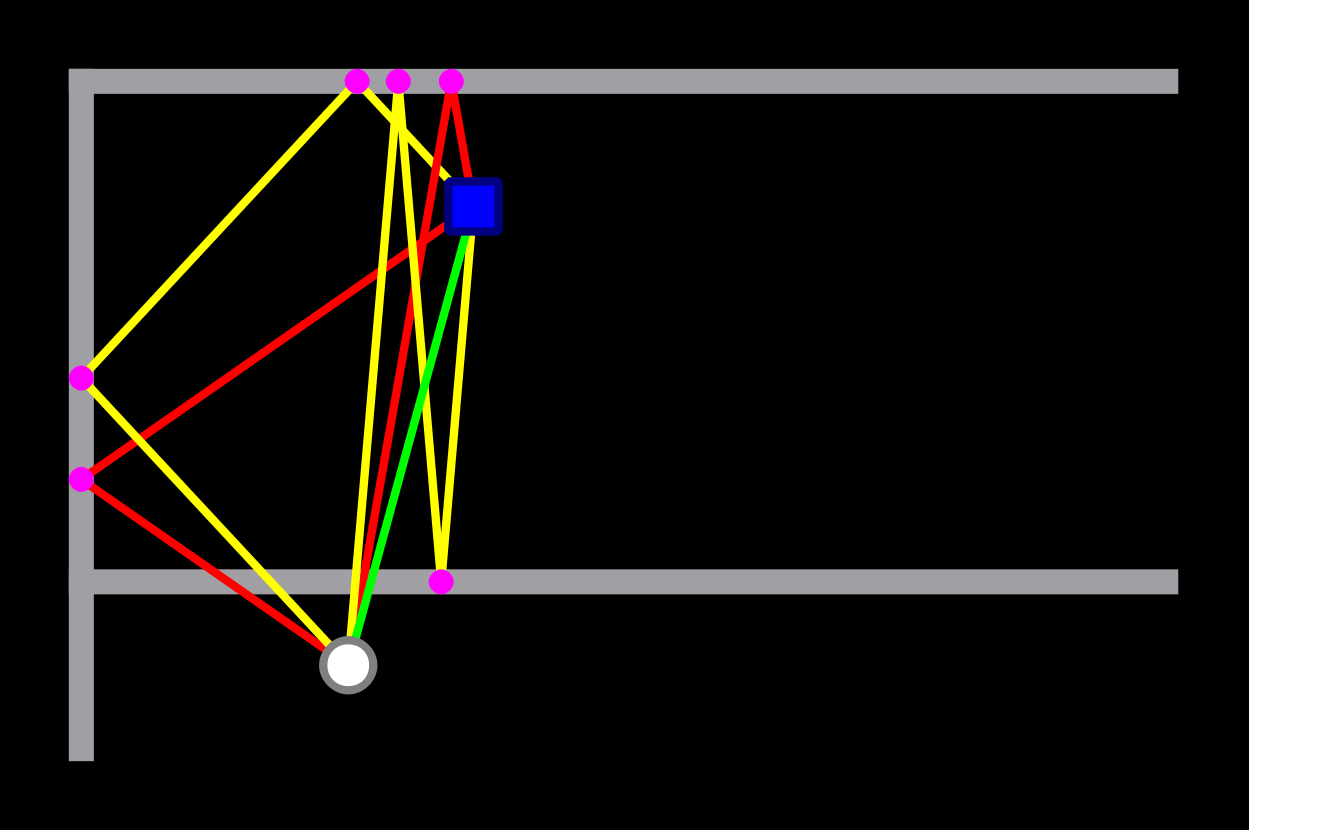
\includegraphics[width=\textwidth]{latex/images/tp4.png}
    \caption{Simulation Ray-Tracing de l'exercice 1, TP4}
    \label{fig:simu-tp4}
\end{figure}
